
%(BEGIN_QUESTION)
% Copyright 2006, Tony R. Kuphaldt, released under the Creative Commons Attribution License (v 1.0)
% This means you may do almost anything with this work of mine, so long as you give me proper credit

A type ``T'' thermocouple is made of the dissimilar metals copper (Cu) and Constantan (C).  Copper is an element while Constantan is an alloy made up of copper and nickel.  Thermocouple ``tables'' published by instrument manufacturers commonly give measurement junction output voltages for different temperatures for an assumed reference junction temperature of 32$^{o}$ F, or 0$^{o}$ C, the freezing point of pure water.  Using such a table, determine the output voltages of a type ``T'' thermocouple constructed from 16 gauge solid wire at the following process temperatures:

$$\includegraphics[width=15.5cm]{i00367x01.eps}$$

\begin{itemize}
\item{} $T_{process}$ = 350$^{o}$ F; Voltmeter voltage = ??? 
\item{} $T_{process}$ = $-$65$^{o}$ F; Voltmeter voltage = ??? 
\item{} $T_{process}$ = 32$^{o}$ F; Voltmeter voltage = ??? 
\item{} $T_{process}$ = 100$^{o}$ C; Voltmeter voltage = ??? 
\end{itemize}

\vskip 10pt

Also determine the standard color codes for type T thermocouple wire:

\begin{itemize}
\item{} Positive conductor:
\item{} Negative conductor:
\item{} Thermocouple-grade jacket:
\item{} Extension-grade jacket:
\end{itemize}

\vskip 20pt \vbox{\hrule \hbox{\strut \vrule{} {\bf Suggestions for Socratic discussion} \vrule} \hrule}

\begin{itemize}
\item{} Explain the rationale of using an ice-water bath for the reference junction.  Also, explain why only one of the reference junction connections is immersed in that bath, while the other (Cu/Cu) is not.
\item{} If the ice-water mixture were to completely melt and rise in temperature, what effect would this have on the measurement accuracy of the thermocouple circuit?  Would it result in a {\it zero} shift, a {\it span} shift, or a change in {\it linearity}?
\end{itemize}

\underbar{file i00367}
%(END_QUESTION)





%(BEGIN_ANSWER)

(From ITS-90 thermocouple table:)

\begin{itemize}
\item{} $T_{process}$ = 350$^{o}$ F; Voltmeter voltage = 8.064 mV 
\item{} $T_{process}$ = $-$65$^{o}$ F; Voltmeter voltage = $-$1.950 mV 
\item{} $T_{process}$ = 32$^{o}$ F; Voltmeter voltage = 0 mV 
\item{} $T_{process}$ = 100$^{o}$ C; Voltmeter voltage = 4.279 mV 
\end{itemize}

\vskip 10pt


Color codes:

\begin{itemize}
\item{} Positive conductor: {\it Blue}
\item{} Negative conductor: {\it Red}
\item{} Thermocouple-grade jacket: {\it Brown}
\item{} Extension-grade jacket: {\it Blue}
\end{itemize}

The last temperature was a ``trick'' question!  You had to convert 100$^{o}$ C into degrees Fahrenheit (212$^{o}$ F), or else look up the answer in a Celsius-indexed table.

\vskip 10pt

The wire size (16 gauge) is extraneous information, included for the purpose of challenging students to identify whether or not information is relevant to solving a particular problem.

%(END_ANSWER)





%(BEGIN_NOTES)


%INDEX% Measurement, temperature: thermocouple (type T)

%(END_NOTES)


